The entire approach has been implemented in the open source process mining framework ProM\footnote{http://promtools.org/} as an interactive plugin in the package \textsc{interactiveLocalizedPlaceAnalysis}. It takes as input an event log, which can be imported from many different data formats via the use of existing conversion plugins, and a Petri net model, with an initial and final marking connected to it. The interactive view is divided into two parts. On the left side, the process model is shown and on the right is a vertical tabbed pane. The first tab is the settings tab from which the algorithm can be started with different parameters. In addition to choosing if log moves should be mapped, is the option to map them but always treat them as incomplete interactions, to respect that they should not have been able to fire. The computation results are added as a new tab. Figure \ref{fig:maininfoview} shows one such tab with the different parts numbered (1)-(7). When selecting a place in the model, the result tab is updated asynchronously with statistics for that place. Switching to a different result tab at that point updates the stats again and makes it easy to compare the differences.

At the top of the result panel is a selection of perspectives (1) which determine the colorization of the model. The perspectives \textit{conformance}, \textit{performance}, \textit{busyness} and \textit{importance} color the places by ranking their respective metrics. The stability perspectives use the relative standard deviation of the metric for the currently selected discretization settings and color based on a capped scale from 0\% to 100\%.
The discretization settings (2) have a slider to select the number of intervals and a toggle to choose if absolute time should be used or the relative time since case start.

Below that (3)-(6) is the place specific information.
The first block of statistics (3) are the properties of the cases that have an interaction with the place. If the average of \emph{Adjacent Case Events} is above $2$, the place is involved in loops. The \emph{Case Duration} is biased compared to the overall case duration average, so it can already be used to compare the performance of different paths in the model. \emph{Sojourn Importance} is the ratio of the total sojourn duration of a case on this place to its entire case duration. The higher the value, the higher is the influence of this place's waiting time on the overall performance.
(4) are the metrics defined in Section \ref{timeintervals} calculated for each case over its whole duration and averaged. (5) are stats of the timeseries of these metrics for the entire place for the currently selected discretization settings of the process duration. The values here are those used in the colorization.
\begin{figure}[H]
    \centering
    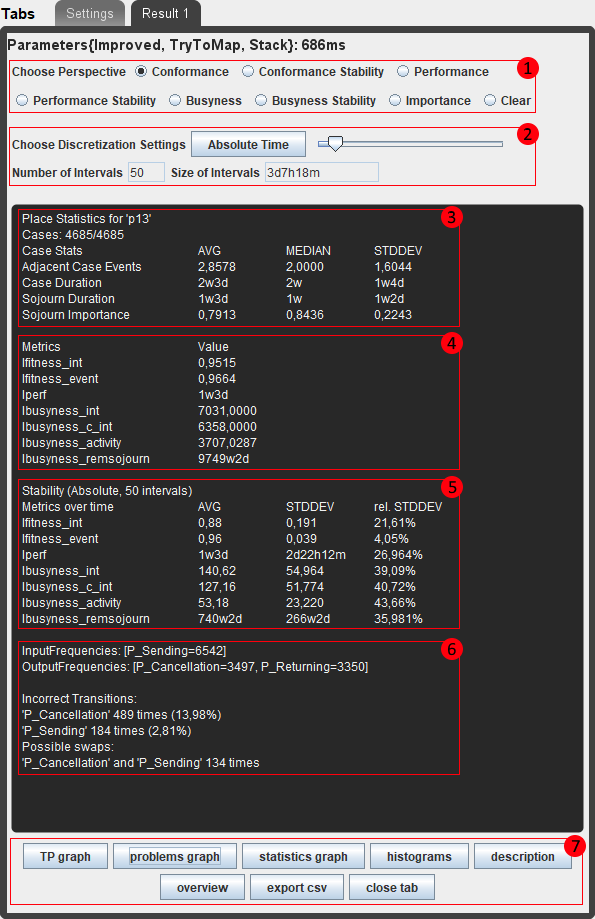
\includegraphics[width=0.7\textwidth]{figures/implementation/main_info_view.png}
    \caption{The main information view}
    \label{fig:maininfoview}
\end{figure}

The other info in this text panel (6) is about the mapped transition executions and how often they are in incomplete interactions. There is also a simple heuristic which tries to detect swapped events by checking if there are two incomplete interactions directly following one another where the first one is just an output transition and the second one an input transition. This obviously only works when log moves are mapped because these swaps cannot occur in sync moves.

Below the text panel are a number of action buttons (7). The \emph{problems graph} shows four selected graphs concerning the conformance at the current place and is intended for visual correlation of the graphs. An example is shown in Figure \ref{fig:probview}. The top left graph displays the number of incomplete interactions per time interval. The top right shows the timeseries of $\func{lfitness_{event}}$ together with its standard deviation over all cases. In the bottom left is a scatterplot of interactions and their durations. The x-axis is the start time of the interaction and the y-axis the duration. Incomplete interactions are colored blue. The bottom right is a timeseries of the frequency of transition executions from incomplete interactions. It can be used to quickly diagnose which activity might be missing or occurring too often when the fitness is low.

The \emph{statistic graph} is a generic view for displaying a graph of any of the presented metrics over time. There are even some more options to be able to experiment with the metrics and variants of them. It also has a button for quickly exporting such a timeseries for external statistical analysis. An example of it is Figure \ref{fig:statview}.
 
 \begin{figure}
    \centering
    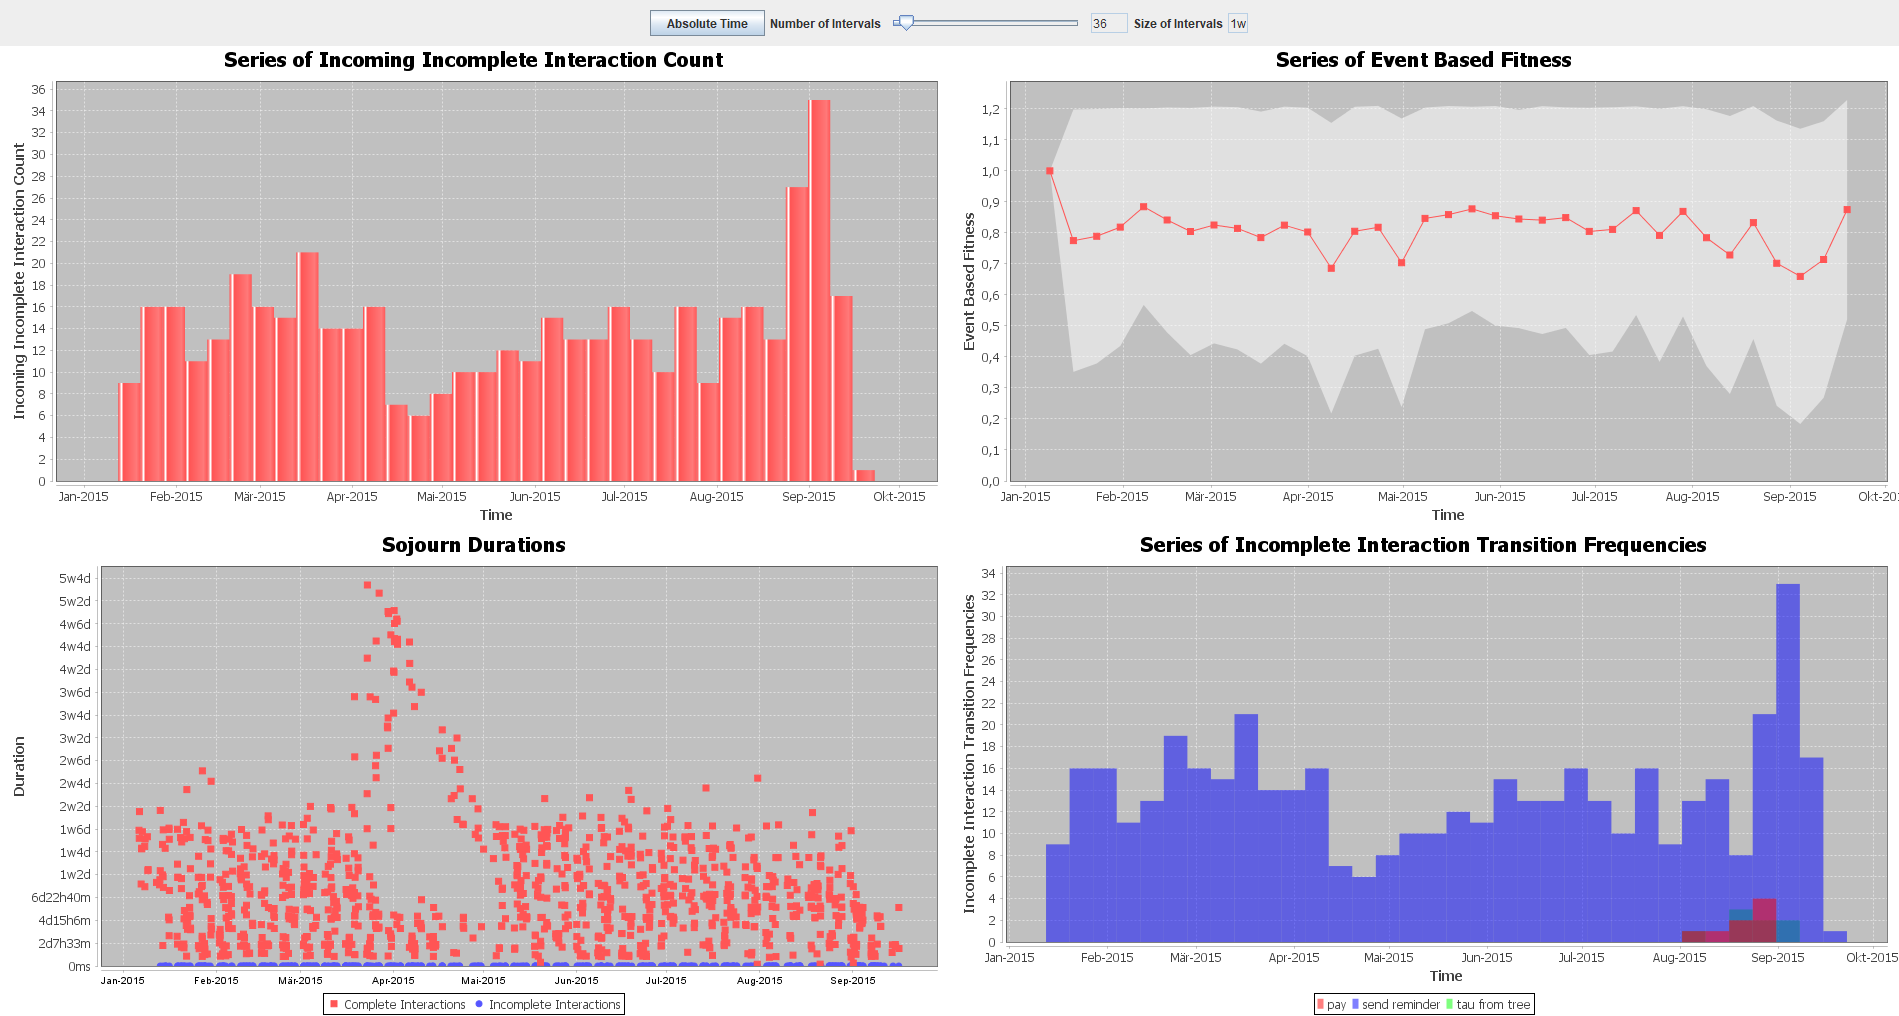
\includegraphics[width=\textwidth]{figures/implementation/problems_view}
    \caption{The problem view}
    \label{fig:probview}
\end{figure}
\begin{figure}
    \centering
    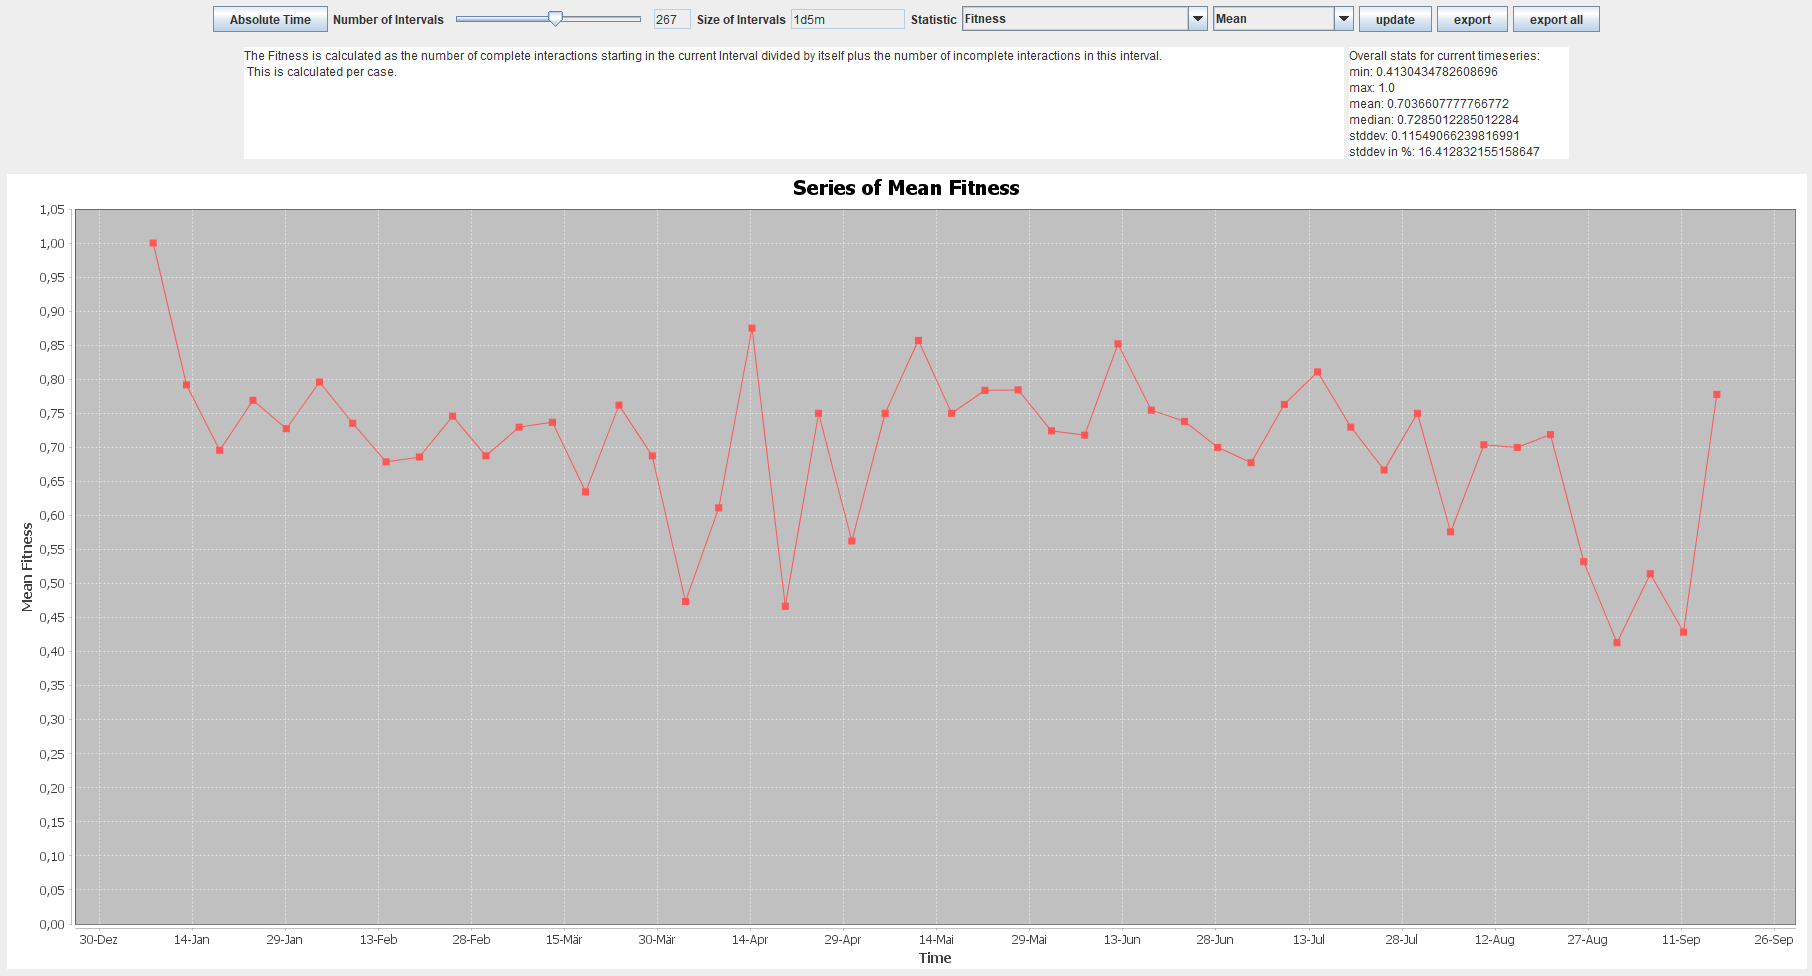
\includegraphics[width=\textwidth]{figures/implementation/genericstatistic_view}
    \caption{The generic statistic view}
    \label{fig:statview}
\end{figure}
\begin{table}
    \centering
    \resizebox{\textwidth}{!}{
    \begin{tabular}{llll}
\hline
StartTime                     & CaseRelativeStartTime & SojournDuration & CaseDuration \\ \hline
2011-10-01 11:45 & 2s                  & 1w1d       & 1w4d     \\       
2012-01-18 11:22 & 2s                  & 4w2d      & 4w2d   \\
2012-02-16 16:24 & 1s                   & 0               & 1s          \\
2012-02-14 20:38 & 9w6d            & 0               & 9w6d   \\

\hline
\hline

lbusyness\_int & lbusyness\_activity & lbusyness\_remsojourn & lperf \\ \hline
309.0 & 133.36   & 484w3d     & 1w4d  \\
1752.0         & 541.87   & 2992w5d     & 1w4d \\
1.0            & 525.0               & 656w2d      & \\
1.0            & 563.0               & 715w6d      & \\

\hline
\hline

lfitness\_int & lfitness\_event    & InputTransition    & OutputTransition \\ \hline
0.99 & 0.99 & O\_SENT            & O\_SENT\_BACK    \\
0.90 & 0.94 & O\_SENT            & O\_CANCELLED     \\
0.0 & 0.0                & O\_SENT            & -   \\
0.0 & 0.0                & + & O\_CANCELLED     \\

\hline
\hline

IsComplete & Iteration & AMOUNT\_REQ  & concept:name \\ \hline
true       & 0         & 20000 & 173688       \\
true       & 0         & 8000 & 201915       \\
false      & 0         & 10000 & 205334       \\
false      & 1         & 5000  & 191797       \\
\hline
\end{tabular}
    }
    \caption{Example for the exportable dataset}
    \label{tab:datasettable}
\end{table}
 Additionally there is also an export button directly on the place information panel in (7). From there it is possible to export a compiled dataset of all interactions with the selected place enhanced with the localized metrics calculated for the duration of the interaction as discussed in Section \ref{alltogether}. Table \ref{tab:datasettable} shows an example for an extracted dataset. The exporter also offers an approximation option for big logs because of the quadratic time complexity of the exact calculations. For the approximation, the stats are calculated once for the selected number of intervals and then via the overlap of the interaction duration and intervals. There are a few other views using histograms and bar charts to present certain simple stats of cases interacting with the place. The \emph{TP graph} button for example shows the graph of token counts of all locally mapped cases with token based replay on the selected place.
 %\begin{figure}
 %    \centering
 %    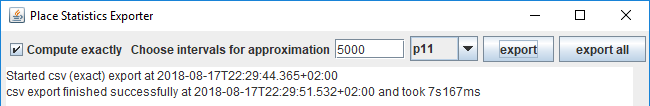
\includegraphics[width = 0.7\textwidth]{figures/implementation/exporter_view.png}
 %    \caption{The exporter view}
 %    \label{fig:expview}
 %\end{figure}
